\chapter{Introductie}
\label{chap:interoperabele_gegevens}
Gegevens die worden gemodelleerd vanuit één enkel perspectief kunnen niet worden gecombineerd of geïntegreerd met andere informatiebronnen of toepassingen en business processen~\cite{interoperability}. Gegevens uit het ene ICT systeem zullen dus niet zomaar bruikbaar zijn in een ander systeem. Bijvoorbeeld, busmaatschappij De Lijn haalt informatie op over wegenwerken uit de database van het Vlaamse Agentschap Wegen en Verkeer. Die informatie kan nuttig zijn om eventuele wegenwerken die het busverkeer hinderen op te sporen. De Lijn kan op basis van deze informatie aanpassingen aanbrengen in de dienstregeling zodat die buslijn\footnote{Busmaatschappij De Lijn gebruikt de term 'lijn' om een bepaalt traject van A naar B aan te duiden.} bedient blijft. In een niet-interoperabel scenario, zal de busmaatschappij voor ieder resultaat uit de wegenwerken database manueel moeten nagaan of lopende werken één of meerdere lijnen doorkruisen of niet. In een wereld waar gegevens tussen de publieke en private sector wel interoperabel zijn, kunnen de systemen van de ene partij overweg met de gegevens van een andere partij. Het computersysteem van De Lijn zal de resultaten van een query, uitgevoerd op de database van Agentschap Wegen en Verkeer, automatisch kunnen interpreteren en het personeel van De Lijn kunnen waarschuwen voor potentiële hinder op een bepaalt deel van een lijn. Daarna kunnen verdere, eventueel manuele, acties worden ondernomen.

Dankzij interoperabiliteit tussen gegevens, krijgen organisaties de mogelijkheid om informatie en kennis te delen op hun eigen manier door middel van gegevensuitwisseling tussen ICT systemen. Het \acrfull{eif} beschrijft een model voor interoperabiliteit dat toepasbaar is op Europese digitale publieke diensten. Met dit programma wilt Europa bouwen aan een naadloze gegevensdoorstroming binnen Europese publieke diensten zoals het Vlaams Agentschap voor Wegen en Verkeer in het voorbeeld hierboven~\cite{neweif}. In de volgende secties van dit hoofdstuk wordt er dieper ingegaan op wat die interoperabiliteit precies is en hoe die kan worden geïmplementeerd.

\section{Semantische interoperabiliteit}
\label{sec:semantische_interoperabiliteit}
Semantische interoperabiliteit gaat over de betekenis en relaties tussen gegevens. Het behandelt zowel syntactische als semantische aspecten. Interoperabiliteit verzekert dat het formaat (syntactisch) en de inhoud (semantisch) van informatie dat werd verzonden, bewaart blijft en wordt begrepen door de ontvanger zoals bedoeld door de verzender. Met andere woorden: Wat werd verzonden, is wat werd begrepen~\cite{neweif}.

Het is niet voor de hand liggend dat iets wordt geïnterpreteerd zoals het werd bedoeld. Als de verzender spreekt over het Sint-Pietersplein, kan dit worden geïnterpreteerd als meerdere verschillende plaatsen of objecten. De ene ontvanger denkt hierbij aan het Sint-Pietersplein in Gent, maar iemand anders denkt direct aan het plein in Vaticaanstad. Parking P10 in Gent heeft dezelfde naam, die bevindt zich onder het Sint-Pietersplein in Gent. Dit probleem doet zich ook voor bij gegevens in een database.

Met behulp van metadata kan duidelijk worden gemaakt wat er precies wordt bedoeld met een bepaalt object. Door relaties tussen objecten te omschrijven kan er nog meer context worden gecreëerd waardoor zowel mens als computer beter kan begrijpen wat er wordt bedoeld door de zender. Om relaties tussen objecten mogelijk te maken zijn er herbruikbare identificatoren nodig die een object uniek identificeren.

\section{Herbruikbare identificatoren}
\label{sec:herbruikbare_ids}
De databases van publieke sectoren bevatten miljoenen objecten. Het is mogelijk dat een zelfde object gebruikt wordt door meerdere verschillende partijen. Neem bijvoorbeeld een fietsenstalling aan een busstation waar reizigers hun fiets kunnen plaatsen als ze de bus nemen, maar waar ook deelfietsen van bijvoorbeeld Velo kunnen worden ontleend. In dat geval wordt het gebruik en de verantwoordelijkheid van dat object uitgebreid naar meerdere partijen: meerdere \glspl{mobop} en diensten van de stad/gemeente die bijvoorbeeld in onderhoud en reparaties voorziet. Gezien dat gedeeld gebruik hebben alle partijen toegang nodig tot de gegevenssets waarin de parameters van dat object lees- en schrijfbaar zijn. Zo een situatie vraagt om interoperabiliteit van gegevens en herbruikbare identificatoren die deze objecten aanduiden. 

Neem als voorbeeld de situatie in figuur~\ref{fig:busstation_labels}. Een busmaatschappij gebruikt de \acrfull{id} van een busstation om aan te duiden waar een bepaalde bus zal stoppen. Datzelfde ID kan door de operator achter de Velo-fietsen worden hergebruikt om aan te duiden dat er een fietsenstalling bij dat busstation te vinden is. Als er elektriciteitsvoorzieningen nodig zijn tot bij het object, kunnen elektriciens door middel van het busstation ID en andere technische informatie precies weten hoe ze te werk moeten gaan. Zo kunnen er bijvoorbeeld verlichtings- en oplaadpunten voor elektrische fietsen worden voorzien en informatie hierover gekoppeld worden aan de ID's van het busstation en fietsenstalling.

\begin{figure}[h]
	\centering
	\begin{subfigure}{\textwidth}
		\centering
		\centerline{
			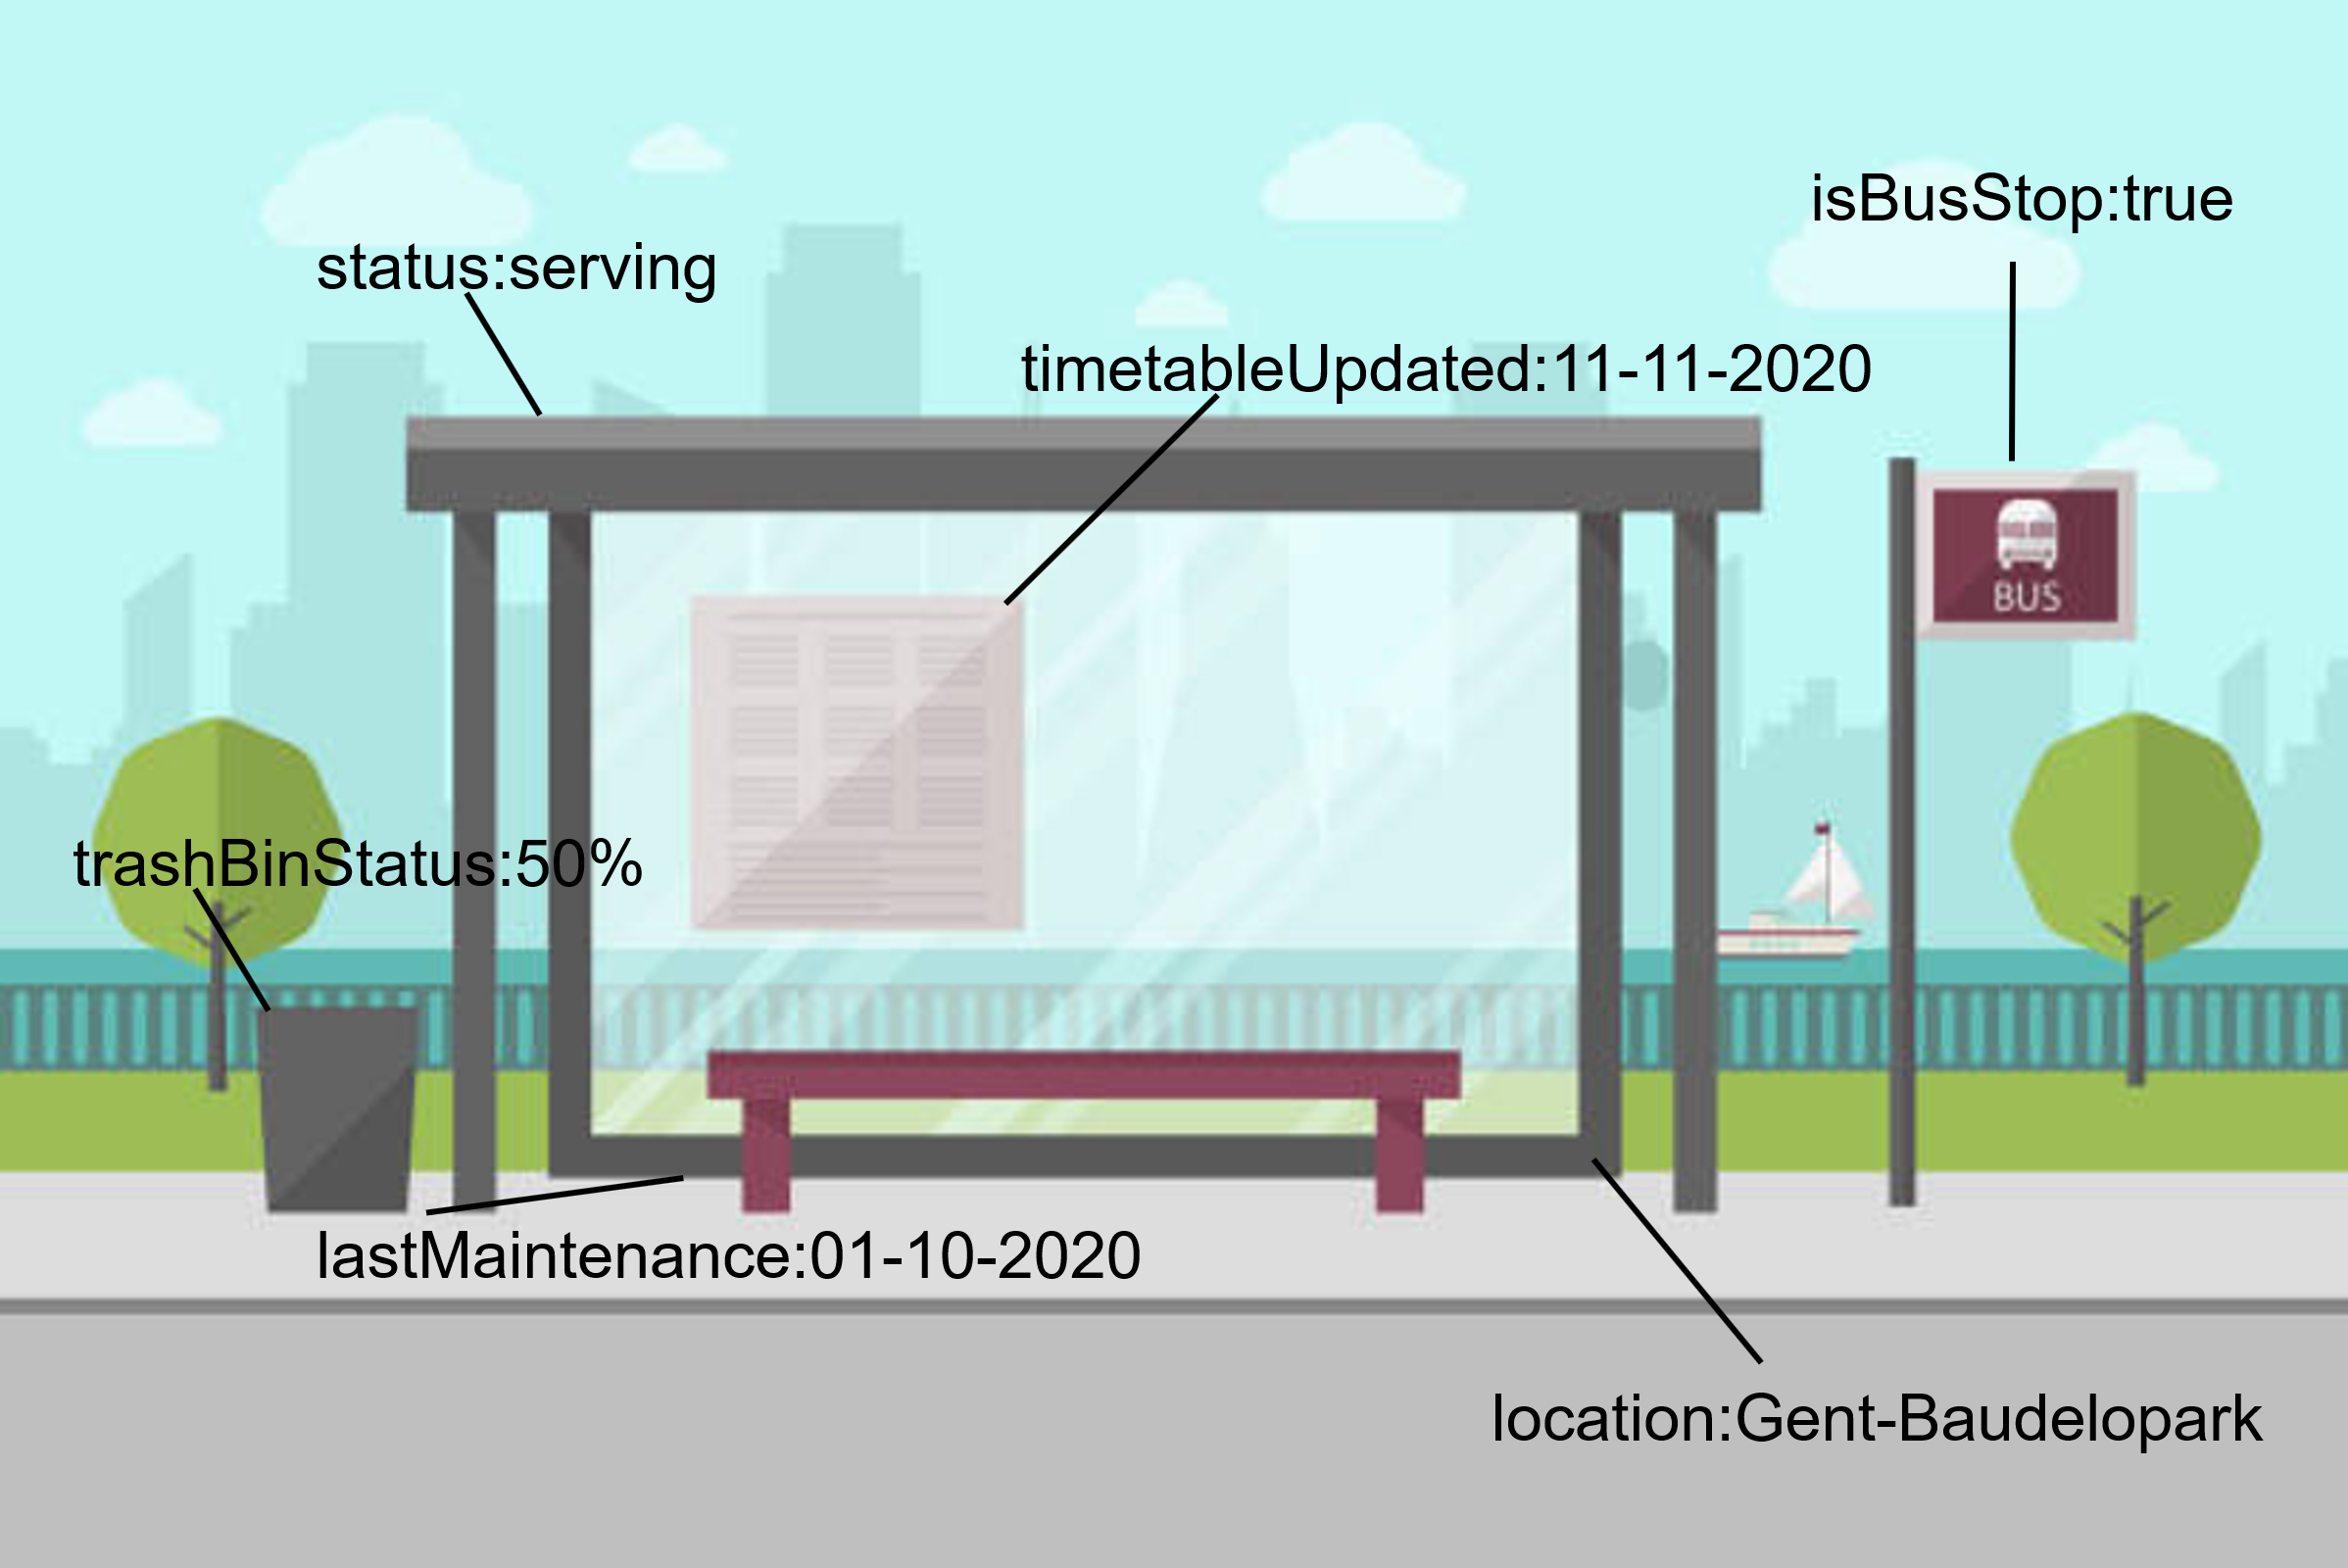
\includegraphics[scale=0.35]{images/busstation_labels.png}
		}
	\end{subfigure}
	\caption{Parameters van een infrastructuur object, gebaseerd op een figuur van istockphoto.com}
	\label{fig:busstation_labels}
\end{figure}

\section{Open Standaarden voor Linkende Organisaties}
\label{sec:OSLO}
Het Vlaams interoperabiliteitsprogramma Open Standaarden voor Linkende Organisaties (OSLO)\footnote{\url{https://data.vlaanderen.be}} is een initiatief van de Vlaamse overheid om hergebruik van gegevens te stimuleren. Het is een van de stappen die Vlaanderen neemt richting een Open Overheid met als doel een nauwere samenwerking te creëren tussen overheid en de privé sector.
Een vorige stap naar open data was het openbaar beschikbaar maken van het Grootschalig Referentiebestand (GRB). Het GRB is een digitale topografische referentiekaart van Vlaanderen waarop alle gebruikers eigen geografische gegevens kunnen aanduiden. Deze locatiegegevens van gebouwen, percelen, wegen en hun inrichting, waterlopen, spoorbanen en het wegennetwerk identificeren miljoenen objecten in Vlaanderen. Dit referentiebestand wordt gebruikt voor onder andere dispatchingtool bij hulpdiensten en het lokaliseren en intekenen van ondergrondse kabels en leidingen~\cite{wat_is_grb}. Sinds het GRB openbaar beschikbaar werd via een gegevensportaal\footnote{\url{http://opendata.vlaanderen.be}} is het gebruik ervan toegenomen van 600 aanvragen naar 2500 per maand~\cite{grb_OD}.

Desondanks de nuttige toepassingen dat het systeem brengt, ondervinden heel wat gebruikers (private partners, bevolking en publieke administratiediensten) moeilijkheden bij het verbinden met en interpreteren van deze open data bronnen. Deze problemen met de interoperabiliteit van gegevens veroorzaken strubbelingen bij het hergebruiken van deze publieke sectorinformatie~\cite{opengovernment}. Om de vraag naar interoperabele gegevens te beantwoorden werd het OSLO programma opgestart dat verder bouwt op de principes van Linked Data en voldoet aan de aanbevelingen uit het \acrshort{eif}.

Het OSLO programma legt de betekenis vast van concepten, woorden en definities en hoe ze te structureren zijn in databases of softwarepakketten. Dankzij deze afspraken, omschreven in datastandaarden, kunnen semantische discussies en misverstanden worden vermeden~\cite{OSLO_handleiding}.

\subsection{OSLO services}
\label{sec:oslo_services}
Informatie Vlaanderen biedt verschillende services aan waarmee het organisaties, in zowel de publieke als privé sector, in het OSLO traject helpt. Samen met de organisatie in kwestie onderzoekt het OSLO-team in hoeverre de aangeleverde informatiemodellen kunnen afgestemd worden op bestaande OSLO-vocabularia. Nadat de noden voor een gegevensmodel in kaart gebracht werden, zal het team een datastandaard (of OSLO-vocabularium) ontwikkelen volgens `Proces \& Methode' van OSLO\footnote{\url{https://data.vlaanderen.be/cms/Proces_en_methode_voor_de_erkenning_van_datastandaarden_v1.0.pdf}}, dat zijn richtlijnen voor het ontwikkelen van nieuwe standaarden binnen OSLO. Nadat er een gepaste datastandaard ontwikkeld of een reeds bestaande standaard toegewezen werd, wordt er ook ondersteuning geboden bij het implementatieproces.

\subsection{Verhoogde interoperabiliteit met OSLO}
Het doel van OSLO is om de gegevensoverdracht tussen verschillende organisaties te versnellen en automatiseren. Dit is nodig omdat de overheid meer dan duizend diensten aanbiedt aan burgers en bedrijven~\cite{OSLO_handleiding}. Deze samenwerking kost tijd en geld doordat gegevens niet interoperabel zijn. Dankzij de hulp van de experten binnen Informatie Vlaanderen, die OSLO mogelijk maken, wordt er aan de nood van interoperabele gegevens tegemoetgekomen. Gegevens worden met OSLO eenduidig gedefinieerd en kunnen beter worden hergebruikt met als resultaat meer samenhang tussen informatie en bijgevolg betere begrijpbaarheid en vindbaarheid ervan.

De huidige doelstelling bestaat erin om zoveel mogelijk gegevenssets te (her)publiceren als \acrshort{lod} met behulp van het OSLO programma. Gegevens rond nieuwe projecten kunnen vanaf nul worden opgebouwd met gestandaardiseerde gegevensmodellen. Reeds bestaande gegevenssets moeten worden omgevormd, zodat het gebruikmaakt van die standaard modellen. Hiervoor zijn tools nodig die verder in deze scriptie worden besproken.

\section{Open Data}
\label{chap:intro}

Tim Berners-Lee, de grondlegger van het \acrfull{www} en oprichter van het \acrfull{w3c}, pleit al jaren voor ``raw data''\footnote{video:  \url{https://www.ted.com/talks/tim_berners_lee_the_next_web} op 10'40''}. Daarmee vraagt hij aan instellingen zoals overheden, onderzoekscentra en bedrijven om hun gegevens openbaar op het internet beschikbaar te stellen zodat het toegankelijk is voor iedereen om er onderzoek op uit te voeren~\cite{tedtalk}. Het openbaar maken van data en het zo ter te beschikking stellen voor iedereen zou wereldverbeterende inzichten moeten opleveren zoals economische groei, efficiënter gebruik van resources en een beter leefwereld voor burgers~\cite{tedtalka}. 
Die inzichten kunnen op een efficiënte manier worden verworven door die open data interpreteerbaar te maken voor machines. Om het Web ook machine-interpreteerbaar te maken werd het concept `Semantisch Web' geïntroduceerd door Tim Berners-Lee. Volgens hem is de meeste inhoud van het web bedoeld voor mensen om te lezen. Computers kunnen goed webpagina's parsen voor layout en routine werk uitvoeren, maar ze hebben geen betrouwbare manier om semantische inhoud te verwerken~\cite{tim_semanticweb}. Computers kunnen, met andere woorden, de bedoeling van de inhoud van een pagina niet interpreteren.

\section{Semantisch Web}
\label{semantisch_web}
Het idee van het Semantisch Web is "om een een Web te weven dat niet enkel documenten aan elkaar linkt, maar ook de betekenis van informatie in die documenten herkent" \cite{frauenfelder}.
Dit Semantisch Web moet gezien worden als een uitbreiding van het huidige Web door een gemeenschappelijke structuur aan te brengen aan de inhoud van webpagina's om zo bij te dragen aan een betere samenwerking tussen mens en machine.~\cite{kuck} Om tot dit Semantisch Web te komen omschreef Tim Berners-Lee vier principes van Linked Data: (i) gebruik URI's om resources te benoemen, (ii) gebruik HTTP URI's zodat die namen kunnen worden opgezocht, (iii) wanneer iemand die URI opzoekt, voorzie dan bruikbare informatie gebruikmakend van standaarden zoals Resource Description Framework, en (iv) voorzie andere URI's zodat er meer resources kunnen worden ontdekt~\cite{designissues}. Wanneer wordt voldaan aan deze vier regels, kunnen gegevens met elkaar in verbinding worden gebracht zoals hyperlinks doen voor documenten op bijvoorbeeld een webpagina.

\subsection{Uniform Resource Identifier}
URI is een begrip dat geïntroduceerd werd door de het IETF\footnote{\url{https://www.ietf.org}} als een internet standaard om een abstracte of fysische resource te identificeren aan de hand van een compacte opeenvolging van karakters~\cite{uri-ietf}. Anders dan de Internationalized Resource Identifier (IRI) kan een URI enkel bestaan uit karakters behorende tot de ASCII karakter-set\footnote{\url{https://theasciicode.com.ar/}}, terwijl deze laatste mag bestaan uit karakters van de Universal coded Character Set (Unicode/ISO 10646)~\cite{ucs}.
Een HTTP URI is een URI dat kan worden gederefereerd met een HTTP-client zodat informatie kan worden opgezocht over de resource geïdentificeerd door de URI. De mogelijkheid tot het dereferen van een URI is een kernprincipe van Linked Data: het kunnen opzoeken van iets dat je niet kent~\cite{verborgh_webfundamental}.

\begin{figure}
	\centering
	\begin{subfigure}{\textwidth}
		\centering
		\centerline{
			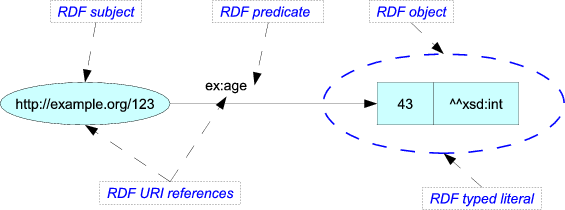
\includegraphics[scale=0.75]{images/rdfexample.png}
		}
	\end{subfigure}
	\caption{Voorbeeld van een \acrshort{rdf} graaf~\cite{rdfgraph_img}}
	\label{fig:rdf_example}
\end{figure}

\section{Resource Description Framework}
\label{sec:rdf}
\acrfull{rdf} is een standaard model om metadata te koppelen aan Web resources en te verwerken. Metadata zijn gegevens over gegevens, en specifiek in deze context zijn het `gegevens die Web resources beschrijven'. Dit model zorgt voor de interoperabiliteit tussen gegevens op het Web door resources te voorzien van eigenschappen en waardes behorend tot die eigenschappen. Een resources is `iets' dat beschreven wordt door een RDF-expressie. Het kan een volledig document zijn, een object in een gegevensset, het kan zelf iets zijn dat niet direct beschikbaar is op het Web bijvoorbeeld jouw fiets of een geprint boek. Een eigenschap is "een specifiek aspect, karakteristiek, attribuut, of relatie dat een resource beschrijft" \cite{rdf}.
Het linken van die metadata gebeurt in de vorm van RDF-triples: een driedelige subject-predicaat-object structuur. Deze gelinkte structuur vormt een gerichte en gelabelde graaf waarbij de takken informatie bevatten (predicaat) over de relatie tussen twee knopen (subject en object)~\cite{rdf_triple}. 
Figuur~\ref{fig:rdf_example} geeft een voorbeeld van hoe zo een graaf er kan uitzien met hieronder een bijhorende tekstuele representatie:

\begin{code}
\begin{minted}[breaklines]{turtle}
@prefix ex:  <http://example.org/> .
@prefix xsd: <https://www.w3.org/2001/XMLSchema#> .

<http://example.org/123> ex:age 43^^xsd:int .
\end{minted}
\caption{RDF-triple in turtle formaat}
\label{code:rdftriple}
\end{code}

Deze RDF-triple bestaat uit de volgende delen:
\begin{table}[h]
\begin{tabular}{|l|l|}
    \hline
    Subject (resource) & <http://example.org/123>\\
    \hline
    Predicaat (eigenschap) & ex:age\\
    \hline
    Object (literal) & 43\\
    \hline
\end{tabular}
\end{table}

\acrshort{rdf} triples kunnen geserialiseerd worden in verschillende vormen. Bovenstaande representatie maakt gebruik van de Turtle syntax\footnote{\url{https://www.w3.org/TR/turtle/}}. Andere serialisatieformaten zijn JSON-LD, RDF/XML, N-triples, ...~\cite{publishingLD}.

In dit voorbeeld wordt het RDF-subject, dat kan hier een persoon zijn, voorgesteld door een \acrshort{uri} die verwijst naar een andere bron die bijvoorbeeld namen van studenten bevat. Met deze triple wordt het subject uitgebreid met een leeftijd. Het RDF-object in figuur~\ref{fig:rdf_example} is geen \acrshort{uri} referentie maar een `RDF typed literal' gebruikt om strings, data en, in dit geval, een getal voor te stellen. Toch kunnen objecten ook verwijzen naar een \acrshort{uri} zoals in deze uitbreiding:

\begin{code}
\begin{minted}[breaklines]{turtle}
@prefix ex:   <http://example.org/> .
@prefix xsd:  <https://www.w3.org/2001/XMLSchema#> .
@prefix foaf: <http://xmlns.com/foaf/0.1/> .

<http://example.org/123> ex:age 43^^xsd:int ;
                         foaf:knows <http://example.org/456> .
\end{minted}
\caption{RDF-triple in turtle formaat -- uitbreiding van Listing \ref{code:rdftriple}}
\label{code:rdftriple_uitbreiding}
\end{code}

Aan het RDF-subject wordt nu door middel van het foaf:knows\footnote{\url{http://xmlns.com/foaf/0.1/}} predicaat een RDF-object gekoppeld dat gedefinieerd werd door een \acrshort{uri} referentie.
In deze uitbreiding werd gebruik gemaakt van een predicaatlijst. Met behulp van het `;'-teken kan het subject worden herhaald waarna predicaat en object kunnen variëren.

\section{RDF-vocabularium}
Om RDF-datamodellen op te bouwen zoals in het voorbeeld hierboven~(Listing \ref{code:rdftriple_uitbreiding}), is er een \gls{ontologie} nodig. \Glspl{ontologie} zijn op voorhand gedefinieerde concepten die relaties kunnen hebben met elkaar, en dat binnen hetzelfde \gls{ontologie} of met andere externe \glspl{ontologie} door verwijzing met een URI. Met behulp van deze documenten kan een gegevensset gemapt worden naar een \acrshort{rdf}-datamodel.
Het publiceren van een document dat een \gls{ontologie} beschrijft, gebeurt opnieuw als door de principes van Linked Data te volgen. De term `ontologie' wordt ook gebruikt om een RDF-vocabularium te benoemen, het duidt echter op een meer complexe collectie van termen. `Vocabularium' wordt in een lossere omgeving toegepast. Alhoewel de twee termen van elkaar verschillen is er geen duidelijk onderscheid over wanneer een dergelijk document een vocabularium of ontologie wordt genoemd~\cite{ontology}.

\subsection{RDF Schema}
RDF Schema (RDFS) is het basis RDF-vocabularium waarmee andere vocabularia kunnen worden gemodelleerd. Het definieert klasses, eigenschappen en datatypes die de basis blokken vormen om andere vocabularia te definiëren~\cite{verborgh_webfundamental}. Het schema definieert concepten in twee namespaces: \url{https://www.w3.org/1999/02/22-rdf-syntax-ns#} en \url{https://www.w3.org/2000/01/rdf-schema#} met respectievelijk de alom aanvaarde prefixen `rdf' en `rdfs'.
Veel gebruikte termen zijn:
\textit{rdfs:Resource} wat een klasse is waarvan alles een instantie is. Bijkomende termen kunnen die instanties verder specialiseren.
\textit{rdfs:Class} is een klasse voor het definiëren van resources die een verzameling van zaken voorstelt.
\textit{rdf:Property} is een klasse voor resources die als predicaat in een RDF-triple kunnen worden gebruikt.
\textit{rdfs:label} dat een eigenschap is dat een voor mensen leesbare naam geeft aan een resource.
\textit{rdf:type} is een eigenschap dat aanduidt dat de resource een instantie is van een klasse.
\textit{rdfs:domain} is een eigenschap dat de klasse van mogelijke subjecten van een eigenschap aantoont. In Listing \ref{code:rdf_example} is \textit{foaf:knows} een eigenschap dat enkel op een instantie van de klasse \textit{foaf:Person} kan worden toegepast.
\textit{rdfs:range} is een eigenschap dat de klasse van mogelijke objecten van een eigenschap aan toont~\cite{verborgh_webfundamental}. In Listing \ref{code:rdf_example} kan het object van de \textit{foaf:knows} eigenschap enkel een object zijn van de klasse \textit{foaf:Person}.

Het codevoorbeeld in Listing~\ref{code:rdf_example} omschrijft het \textit{foaf:knows} predicaat uit Listing~\ref{code:rdftriple_uitbreiding}. Bij het definiëren van dit concept wordt gebruik gemaakt van andere \glspl{ontologie} (hier rdf, rdfs en owl) door via \acrshort{uri}s te verwijzen naar concepten uit die \glspl{ontologie}. Door het concept `knows' te interpreteren wordt duidelijk dat het om een eigenschap gaat dat moet gebruikt worden binnen het domein \textit{foaf:Person}. Het object dat de eigenschap aanvaardt, wordt aangeduid met de `range' eigenschap en is in dit voorbeeld ook de klasse \textit{foaf:Person}.

\subsection{Ontology Web Language}
Terwijl RDFS vooral de basis concepten voor relaties definieert, kan het Ontology Web Language (OWL) vocabularium gezien worden als een uitbreiding van RDFS doordat het meer geavanceerde concepten definieert.
OWL wordt gebruikt om klasses, eigenschappen en individuen verder te specificeren~\cite{verborgh_webfundamental}.
De termen `instantie' en `individu' hebben hier elk een andere betekenis. Een klasse gedefinieerd door ontwikkelaars is een \textit{instantie} van de bestaande \textit{owl:Class} klasse. Terwijl een een \textit{individu} een instantie is van de (nieuwe) gedefinieerde klasse afgeleid van \textit{owl:Class}~\cite{owl}.
In Listing~\ref{code:rdf_example} zijn de klassen \textit{ex:Dier} en \textit{ex:Kat} instanties van \textit{owl:Class} en is \textit{ex:sam01} een individu van de klasse \textit{ex:Kat}.

\begin{code}
\begin{minted}[breaklines]{turtle}
@prefix ex:  <https://example.org/rdf#>
@prefix owl: <https://www.w3.org/2002/07/owl#> .
@prefix rdf: <http://www.w3.org/1999/02/22-rdf-syntax-ns#> .
@prefix rdfs: <http://www.w3.org/2000/01/rdf-schema#> .
@prefix foaf: <http://xmlns.com/foaf/0.1/> .

ex:Dier a owl:Class ;
        rdfs:label "dier" ;
        rdfs:comment "Een levend wezen dat geen mens en plant is." .
        
ex:Kat  a ex:Dier ;
        rdfs:label "kat" ;
        rdfs:comment "Een gewerveld dier behorend tot de groep van katachtigen" .
        
ex:sam01 a ex:Kat ;
         foaf:name "Sam" .

foaf:knows a rdf:Property,
             owl:ObjectProperty ;
            rdfs:comment "A person known by this person (indicating some level of reciprocated interaction between the parties)." ;
            rdfs:domain foaf:Person ;
            rdfs:isDefinedBy foaf: ;
            rdfs:label "knows" ;
            rdfs:range foaf:Person .
\end{minted}
\caption{Voorbeeld van een zelf gedefinieerde instantie en individu en een instantie van het FoaF RDF-vocabularium}
\label{code:rdf_example}
\end{code}

\section{SPARQL}
SPARQL is een query-taal om gegevens uit een RDF-gegevensset op te vragen door een `basic graph pattern' (BGP) op te bouwen. Zo een BGP bestaat uit een collectie van triplet-patronen die lijken op de RDF-tripletten uit sectie~\ref{sec:rdf}. Het verschil is hier dat de URI van het subject, predicaat of object kan worden vervangen door een variabele. Er is een match tussen de BGP en een subgraaf van de gegevensset als RDF-termen kunnen gesubstitueerd worden voor de variabelen uit de GBP. Het resultaat is een RDF-graaf gelijkaardig aan die van de subgraaf~\cite{sparql}. Een simpel voorbeeld met als gegevensset de RDF-grafen uit Listing~\ref{code:rdf_example} is die  in Listing~\ref{code:sparql} met resultaat `name: "Sam"'.

\begin{code}
\begin{minted}[breaklines]{sparql}
@prefix ex:  <https://example.org/rdf#>
@prefix foaf: <http://xmlns.com/foaf/0.1/> .

SELECT ?name 
WHERE{
    ?s a ex:Kat .
    ?s foaf:name ?name .
}

\end{minted}
\caption{Voorbeeld SPARQL-query met als datasource Listing~\ref{code:rdf_example}}
\label{code:sparql}
\end{code}

SPARQL heeft vier query vormen die een resultaat teruggeven. (i) `SELECT' geeft de variabelen uit de BGP terug die konden worden gesubstitueerd met RDF-termen in de graaf uit de RDF-gegevensset. (ii) De `CONSTRUCT'-clausule creëert tripletten die aan de condities van de clausule voldoen, (iii) terwijl de `ASK'-clausule checkt of de gegevens die worden gequeryd wel bestaan. (iv) De `DESCRIBE'-clausule geeft informatie terug over een resource~\cite{verborgh_webfundamental}.

\section{Vijfsterrenmodel}
\label{sec:linked_open_data}
Om mensen te stimuleren kwalitatief goede Linked Data te publiceren, ontwikkelde Tim Berners-Lee een vijfsterrenmodel. 
Linked Open Data krijgt vijf sterren wanneer het voldoet aan een aantal voorwaarden: (i) de gegevens moeten online onder een open licentie beschikbaar zijn, (ii) de gegevens moeten machine-leesbaar zijn en mogen dus géén scan van een document zijn, (iii) daar bovenop moet het in een open bestandsformaat beschikbaar zijn (bijvoorbeeld csv in plaats van excel), (iv) bovendien moet het gebruikmaken van de w3c\footnote{\url{https://www.w3.org/standards/}} standaard bv. \acrfull{rdf} zodat anderen naar de dataobjecten kunnen verwijzen. (v) De gegevens zelf moeten ook verwijzen naar gegevens van anderen zodat er meer context kan gecreeërd worden.
In de inleiding van dit hoofdstuk werd duidelijk dat overheden en bedrijven meer gegevens onder een open licentie moeten delen. Dit geldt natuurlijk niet voor belangrijke gegevens die intern moeten blijven of voor persoonlijke gegevens. Linked Data kan even goed vijf sterren hebben zonder dat het onder een open licentie moet worden gepubliceerd. Indien er echter over Linked Open Data gesproken wordt, moet het uiteraard wel `open' zijn om sterren te kunnen verdienen.

\section{Probleemstelling en doel van de masterproef}
\label{sec:problem}
De non-interoperabiliteit van gegevens van de publieke sector diensten resulteert in een moeilijke samenwerking tussen partijen die gegevens van elkaar gebruiken. 
Het herpubliceren van die gegevens als Linked Open Data en hergebruiken van identificatoren kan de interoperabiliteit tussen gegevens verhogen.
Meer specifiek moeten de gegevens interoperabel zijn met de andere gegevens van de Vlaamse overheid. 
Hieraan wordt, op dit moment van schrijven, in Vlaanderen al volop gewerkt met het Vlaams interoperabiliteitsprogramma `Open Standaarden voor Linkende Organisaties' of kortweg: OSLO\footnote{https://data.vlaanderen.be/}. 
Dit programma ontwikkeld vocabularia om gegevens van (Belgische) overheden en bedrijven te publiceren als \acrshort{lod}. 
De doelstelling van deze masterproef is om ook gegevens van \glspl{mobop} mee in het OSLO-traject te krijgen door een RDF-vocabularium te voorzien waarin de gegevens OSLO-conform kunnen worden gepubliceerd en methodes aan te reiken bestaande gegevens te mappen op dat nieuwe vocabularium.
Deze twee stappen vormen de `oprit' de OSLO-pijplijn en wordt verder in deze scriptie de `on-boarding' van gegevens genoemd. Na deze on-boarding fase kunnen de gegevens verder hun weg vinden doorheen de pijplijn naar onder andere archivering en kunnen 
queries opgebouwd worden die meerdere thematisch verschillende gegevenssets aanspreken.

In deze masterproef zullen de gegevens van \glspl{fietsdeelop} Blue Bike en Velo als aanknopingspunt worden onderzocht. Als eerste contributie wordt bekeken of er standaard specificaties zijn waaruit concepten en structuren kunnen worden hergebruikt in een nieuw RDF-vocabularium dat zal worden ontwikkeld. 
Dat vocabularium moet een connectie hebben met de bestaande OSLO-vocabularia zodat de gegevens interoperabel zijn met andere gegevens van de Vlaamse overheid. Om die connectie te maken ga ik opzoek naar een OSLO-vocabularium met concepten die aansluiten bij de termen die reeds in gegevenssets rond fietsdeelsystemen worden gebruikt.
Ter demonstratie worden gegevens met behulp van het ontwikkelde vocabularium gemapt naar een \acrshort{rdf}-gegevensset en gepubliceerd als \acrlong{lod}. Tijdens het onderzoek en de implementatie moet er zo generiek mogelijk te werk worden gegaan zodat in een volgende fase andere types vervoermiddelen kunnen worden geïmplementeerd. Als laatste contributie moeten er oplossingen worden aangeboden aan de operatoren om hun gegevens te herpubliceren gebruikmakend van het ontwikkelde vocabularium zonder dat dit een extra last brengt bij de publicatie van de gegevens.

\chapter{State of the art}

Er zijn specificaties (GBFS\footnote{\url{https://github.com/NABSA/gbfs}}, GTFS\footnote{\url{https://developers.google.com/transit/gtfs/reference}}, MDS\footnote{\url{https://github.com/openmobilityfoundation/mobility-data-specification/tree/master}}) die een zo generiek mogelijk gegevensmodel voorstellen zodat \glspl{mobop} hun gegevens op een interoperabele manier kunnen publiceren. Helaas zijn deze specificaties volgens het sterrenschema van Tim Berners-Lee geen vijf sterren waard. De gepubliceerde gegevens voldoen daarom niet aan de concepten van het European Interoperability Framework door tekortkomingen beschreven in secties~\ref{sec:GBFS} en \ref{sec:ngsi}.

Daarnaast bestaan er al \glspl{ontologie} (Mobivoc\footnote{\url{http://schema.mobivoc.org}} en OSLO mobiliteit: trips \& aanbod\footnote{\url{https://data.vlaanderen.be/doc/applicatieprofiel/mobiliteit-trips-en-aanbod}}) waarmee gegevens van \glspl{mobop} als \acrshort{lod} kunnen worden gepubliceerd. Deze vocabularia hebben beperkingen die omschreven worden in secties~\ref{sec:trips&aanbod} en \ref{sec:mobivoc} waardoor ze geen volledige oplossing bieden voor fietsdeeloperator gerelateerde gegevens. Wel kunnen deze \glspl{ontologie} gebruikt worden als basis voor een nieuwe ontologie of kan er een uitbreiding voor gemaakt worden. 

\section{General Bikeshare Feed Specification}
\label{sec:GBFS}
GBFS is een open standaard voor deelmobiliteit dat in een uniform formaat real-time gegevens publiceert. Het voordeel aan deze specificatie is dat het om een open standaard gaat en bruikbaar is door iedereen en voor verschillende toepassingen. Tussen systemen die gebruikmaken van GBFS is er interoperabiliteit, maar daarbuiten niet. Wie met de standaard werkt, wordt verplicht de gegevensset te publiceren in het JSON-gegevensformaat. Hierdoor blijven semantische discussies over de betekenis van de gebruikte sleutels in het model mogelijk. Dit veroorzaakt een gebrek aan interoperabiliteit bij gegevensoverdracht tussen systemen buiten de grenzen van GBFS, zoals diensten van overheden. Zonder mapping kunnen andere systemen niet aansluiten op deze gegevens gepubliceerd in de open standaard. Daarnaast vereist de standaard geen herbruikbare identificatoren waardoor de gegevens van objecten niet uitbreidbaar zijn. 

Dankzij het gebruikte JSON-formaat van GBFS zijn gegevens die onder een open licentie worden gepubliceerd drie sterren  (\ast \ast \ast) waard volgens het vijfsterrenmodel.
Er kan hier echter niet gesproken worden over Linked Data gezien
er geen gebruik wordt gemaakt van open standaarden van w3c (RDF) en de gegevens niet op te vragen zijn met SPARQL. 

Toch lijkt het model van deze specificatie een goed startpunt te zijn om gegevens van fietsdeeloperatoren in te publiceren. GBFS bewees zichzelf reeds doordat het, op het moment van schrijven,  door verschillende operatoren wereldwijd op 452 plaatsen wordt gebruikt~\cite{GBFS_systems}. Operatoren die gebruikmaken van de standaard hier in België zijn: Donkey Republic (actief in Gent) en Bird (actief in Antwerpen). De lijst~\footnote{\url{https://github.com/NABSA/gbfs/blob/master/systems.csv}} bevat voornamenlijk operatoren die deelfietsen aanbieden. Toch zijn er ook operatoren die andere voertuigen aanbieden volgens hetzelfde \gls{deeleconomie} principe en met hetzelfde gegevensmodel. Vervoermiddel-specifieke gegevens zoals het aantal beschikbare voertuigen en docks van een bepaald type, worden niet rechtstreeks met een eigenschap toegevoegd aan een stations-object. In plaats daarvan heeft een stations-object een array met objecten die zich van elkaar onderscheiden door de toevoeging van een eigenschap met het type vervoermiddel waartoe deze informatie hoort.
De GBFS-standaard voorziet objecten met eigenschappen voor informatie over stations en hun real-time status, voertuigen en hun status en andere systeem eigen informatie~\footnote{\url{https://github.com/NABSA/gbfs/blob/master/gbfs.md}}.

\section{NGSI}
\label{sec:ngsi}
NGSI\footnote{\url{https://fiware-ges.github.io/orion/api/v2/stable/}} is een verzameling van gegevensmodellen voor uiteenlopende toepassingen: Smart Cities, Smart Agrifood, Smart Environment, Smart Sensoring, Smart Enery, Smart Water en andere. Een van de gegevensmodellen dat FIWARE, de organisatie achter de specificatie, ontwikkeld heeft is `Bike Hire Docking Station'. Net zoals GBFS kan dit gegevensmodel worden gebruikt door fietsdeeloperatoren om hun gegevens te publiceren in JSON-formaat. Het verschil met GBFS is dat iedere eigenschap nog extra eigenschappen heeft. Die `sub-eigenschappen' houden metadata bij voor hun eigenschap, zoals een timestamp. Eén van die sub-eigenschappen, misschien wel de belangrijkste, is de `value'-eigenschap die de waarde van zijn super-eigenschap bijhoudt. Verdere vergelijkingen tussen NGSI en GBFS vallen buiten de scope van deze scriptie.

Deze specificatie kan met dezelfde argumenten als die voor GBFS worden beoordeeld met drie sterren (\ast \ast \ast) volgens het vijfsterrenmodel.

\section{NGSI-LD}
\label{sec:ngsi-ld}
NGSI-LD is gebasseerd op JSON-LD\footnote{\url{https://json-ld.org/}} en is de Linked Data versie van de klassieke NGSI gegevensmodellen. JSON-LD kan door middel van het toevoegen van een `@context'-object een JSON gegevensset beschikbaar maken als Linked Data, querybaar met een SPARQL query.
Een NGSI-LD gegevensmodel zit anders in elkaar dan een klassiek RDF-model door het invoeren van sub-eigenschappen. Daarom introduceert FIWARE de NGSI-LD core context\footnote{\url{https://uri.etsi.org/ngsi-ld/v1/ngsi-ld-core-context.jsonld}} om termen te mappen op URI's. In de gegevensmodellen context\footnote{\url{https://fiware.github.io/data-models/context.jsonld}} van NGSI, worden URI's beschreven om de termen die eigen zijn aan de NGSI modellen te mappen op URI's waardoor er binnen het NGSI-LD ecosysteem interoperabiliteit is. De URI's zijn echter geen HTTP URI's, het is niet mogelijk om bijvoorbeeld de URI \url{https://uri.fiware.org/ns/data-models#availableBikeNumber} te derefereren. Volgens de vier principes van Linked Data (sectie \ref{semantisch_web}) is dit wel een vereiste waardoor het LD gedeelte in NGSI\textbf{-LD} niet op zijn plaats staat. NGSI-LD kan dus geen Linked Data genoemd worden omdat de URI's geen bruikbare informatie leveren over de predicaten.

\section{OSLO mobiliteit: trips \& aanbod}
\label{sec:trips&aanbod}
De OSLO mobiliteit: trips \& aanbod specificatie is onderdeel van het OSLO programma beschreven in sectie~\ref{sec:OSLO}. Gezien de aard van OSLO kan een gegevensset gepubliceerd volgens dit RDF-vocabularium worden beoordeeld met vijf sterren (\ast \ast \ast \ast \ast). Het vocabularium voorziet allerhande termen voor gegevensuitwisseling over door personen uitgevoerde reizen en de mobiliteitsdiensten die ze daarvoor ter beschikking hebben~\cite{oslomobiliteit}. Dit lijkt een goed kandidaat-gegevensmodel waarmee gegevens van fietsdeeloperatoren kunnen worden gepubliceerd. De klassen en eigenschappen beschreven door het vocabularium zijn echter beperkt. De RDF-termen beschrijven hoofdzakelijk zeer low level concepten en begrippen zoals aanbieder, mobiliteitsdienst, prijsplan, reiziger, route enz...~\footnote{\url{https://data.vlaanderen.be/doc/applicatieprofiel/mobiliteit-trips-en-aanbod\#overview}} Om gegevens van fietsdeeloperatoren te publiceren is er meer nood aan RDF-termen gelijkaardig aan de properties van GBFS.

\section{MobiVoc: Open Mobility Vocabulary}
\label{sec:mobivoc}
Deze specificatie maakt ook gebruik van RDF. Gegevens gepubliceerd met dit RDF-vocabularium hebben potentieel om vijf sterren (\ast \ast \ast \ast \ast) waard te zijn. Mobivoc profileert zich als een vocabularium voor toekomstgerichte mobiliteit. Hiermee lijkt ook dit vocabularium een goede kandidaat voor het publiceren van gegevens van fietsdeeloperatoren als LOD. Het vocabularium bevat een ruim assortiment aan RDF-termen zoals `bicycle parking station' dat een subklasse is van `parking facility'. Daarnaast bevat het ook termen om eigenschappen van voertuigen en stations te modelleren zoals de real-time capaciteit. 

Hetgeen dat hier mist is een connectie met OSLO zodat er kan gelinkt worden naar reeds bestaande gegevenssets in Vlaanderen. Op die manier kunnen nieuwe en bestaande fietsenstallingen voor deelfietsen gelinkt worden aan adressen, plaatsen of openbare gebouwen die reeds als LOD objecten ter beschikking worden gesteld met de OSLO-vocabularia. 